\section{one-loop result for unpolarized quasi-quark distribution}

In this section, we consider the one-loop correction in the case of unpolarized quasi-quark distribution $\tilde q(x, \mu^2, P^z)$. The one-loop computation for non-singlet quark distribution is similar to QED because the non-Abelian property
does not enter in the non-singlet case.

Since the one-loop result is gauge-invariant, we can perform the calculation in any gauge. The simplest choice is the axial gauge $A^z=0$~\cite{axial}, as in this gauge the gauge link in Eq.~(\ref{qUnpolDef}) becomes unity. In the axial gauge, the relevant Feynman diagrams are shown in Fig. 1, where the non-local operator
is depicted as a dashed line. The diagrams contain UV, soft and collinear divergences. We use the quark mass $m$ to regulate the collinear divergence. The soft divergence
is expected to cancel between the diagrams. The UV divergence is regulated
by a transverse-momentum cut-off. Of course this cut-off violates rotational symmetry. However, it
is expected to yield the correct leading-logarithmic behavior.

\begin{figure}[htbp]
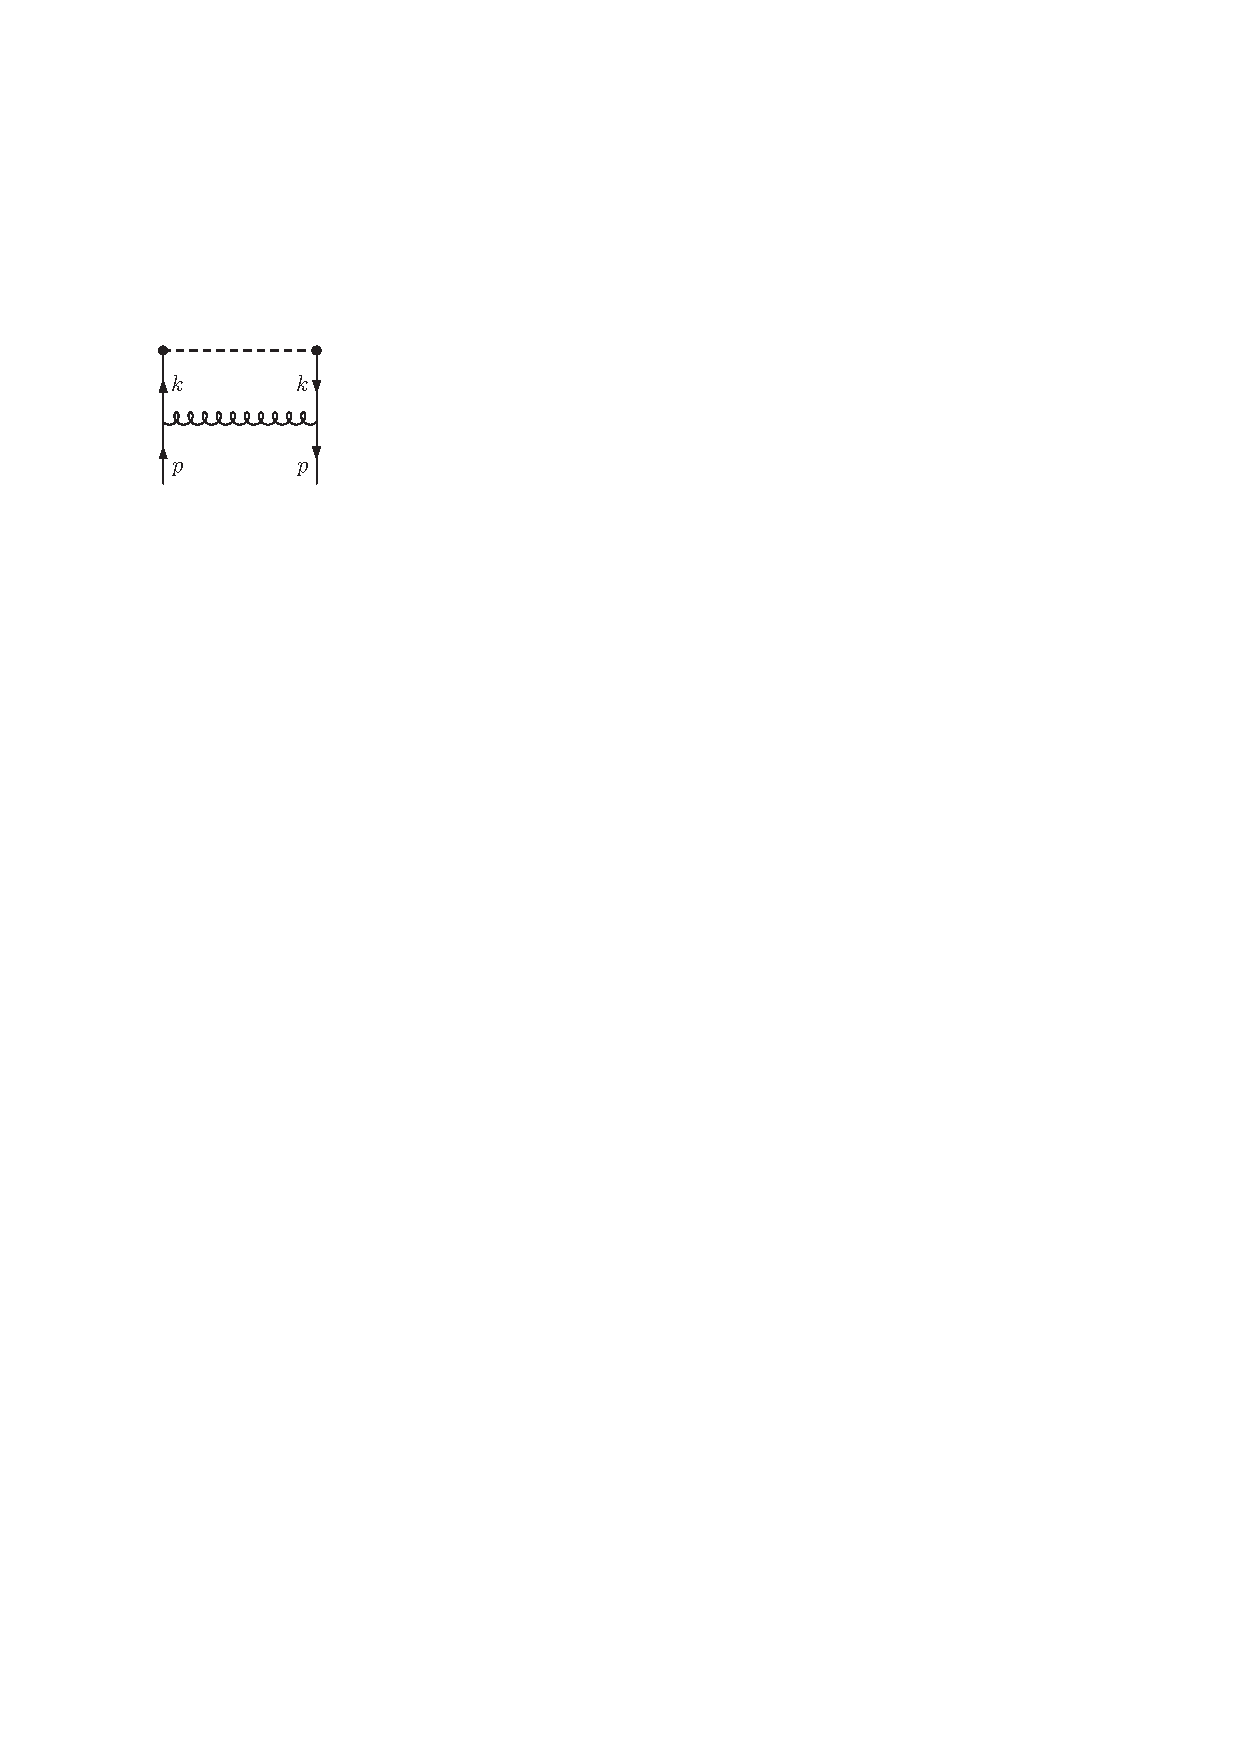
\includegraphics[width=0.2\textwidth]{images/vertex.pdf}
\hspace{10em}
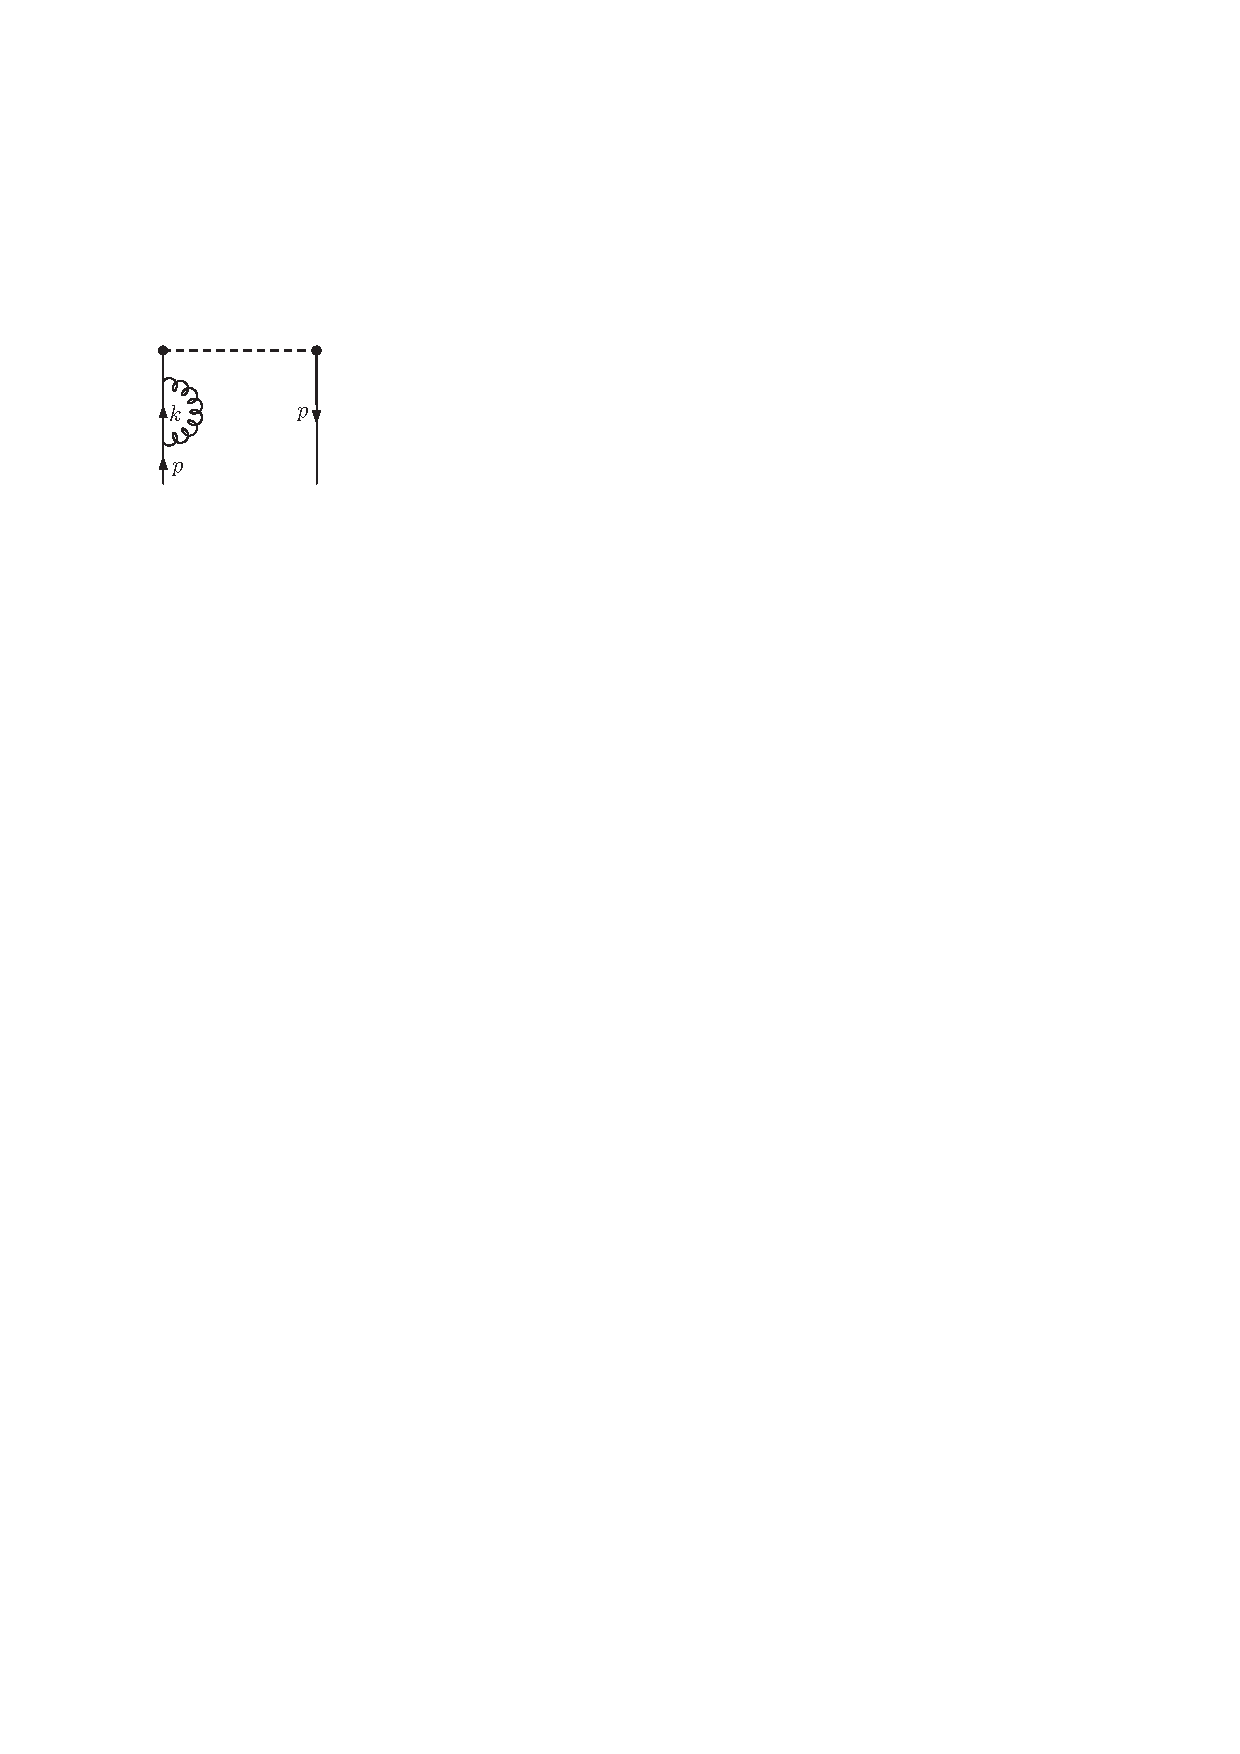
\includegraphics[width=0.2\textwidth]{images/self.pdf}
\caption{One loop corrections to quasi quark distribution.}
\label{onelooppdf}
\end{figure}

The one-loop diagrams generate the following result
\begin{equation}
                    \tilde q(x, \mu^z, P^z) = (1+\tilde Z^{(1)}_F+\dots) \delta(x-1) + \tilde q^{(1)}(x) + \dots
\end{equation}
with
\begin{align}\label{unpolvertexnoexp}
\tilde q^{(1)}(x)&=\frac{\alpha_S C_F}{2\pi} \left\{ \begin{array} {ll} \frac{1+x^2}{1-x}\ln \frac{x(\Lambda(x)-x P^z)}{(x-1)(\Lambda(1-x)+P^z(1-x))}+1-\frac{x P^z}{\Lambda(x)}+\frac{x\Lambda(1-x)+(1-x)\Lambda(x)}{(1-x)^2 P^z}\ , & x>1\ , \\
\ \\
\frac{1+x^2}{1-x}\ln\frac{(P^z)^2}{m^2}+\frac{1+x^2}{1-x}\ln \frac{4x(\Lambda(x)-x P^z)}{(1-x)(\Lambda(1-x)+(1-x)P^z)}-\frac{4x}{1-x}+1-\frac{x P^z}{\Lambda(x)}\ & \\
+\frac{x\Lambda(1-x)+(1-x)\Lambda(x)}{(1-x)^2 P^z}\ , & 0<x<1\ , \\
\ \\
\frac{1+x^2}{1-x}\ln \frac{(x-1)(\Lambda(x)-x P^z)}{x(\Lambda(1-x)+(1-x)P^z)}-1-\frac{x P^z}{\Lambda(x)}+\frac{x\Lambda(1-x)+(1-x)\Lambda(x)}{(1-x)^2P^z}\ , & x<0 \end{array} \right.
\end{align}
for finite $P^z$, where $\Lambda(x)=\sqrt{\mu^2+x^2 (P^z)^2}$ and the logarithm with collinear divergences
is related to the standard Altarelli-Parisi kernel~\cite{AP}. The wave function renormalization correction
depends on the momentum $P^z$ as well
\begin{align}\label{selfnoexp}
\tilde Z^{(1)}_F&=\frac{\alpha_S C_F}{2\pi} \int dy \left\{ \begin{array} {ll} -\frac{1+y^2}{1-y}\ln \frac{y(\Lambda(y)-y P^z)}{(y-1)(\Lambda(1-y)+P^z(1-y))}-1-\frac{y\Lambda(1-y)+(1-y)\Lambda(y)}{(1-y)^2 P^z}\ & \\
+\frac{y^2 P^z}{\Lambda(y)}+\frac{y(1-y)P^z}{\Lambda(1-y)}+\frac{\Lambda(y)-\Lambda(1-y)}{P^z}\ , & y>1\ , \\
\ \\
-\frac{1+y^2}{1-y}\ln\frac{(P^z)^2}{m^2}-\frac{1+y^2}{1-y}\ln \frac{4y(\Lambda(y)-y P^z)}{(1-y)(\Lambda(1-y)+(1-y)P^z)}+\frac{4y^2}{1-y}+1\ & \\
-\frac{y\Lambda(1-y)+(1-y)\Lambda(y)}{(1-y)^2P^z}+\frac{y^2 P^z}{\Lambda(y)}+\frac{y(1-y)P^z}{\Lambda(1-y)}+\frac{\Lambda(y)-\Lambda(1-y)}{P^z}\ , & 0<y<1\ , \\
\ \\
-\frac{1+y^2}{1-y}\ln \frac{(y-1)(\Lambda(y)-y P^z)}{y(\Lambda(1-y)+(1-y)P^z)}+1-\frac{y\Lambda(1-y)+(1-y)\Lambda(y)}{(1-y)^2P^z}\ & \\
+\frac{y(1-y)P^z}{\Lambda(1-y)}+\frac{y^2 P^z}{\Lambda(y)}+\frac{\Lambda(y)-\Lambda(1-y)}{P^z}\ , & y<0\ . \end{array} \right.
\end{align}
It is easy to check that the result obeys the vector current conservation condition
\begin{equation}
  \int^{+\infty}_{-\infty} dx\, \tilde q(x, \mu^2, P^z) =1
\end{equation}
to one-loop order. Since the constituent of the quark in a quasi-distribution does not have a parton interpretation,
the parton momentum fraction extends from $-\infty$ to $+\infty$. However, it is interesting to see that the collinear divergence
exists only for $0<x<1$.


In field theory calculations, one often takes the ultraviolet cut-off to be larger than any other scale
in the problem. In other words, one shall take the limit $\mu\rightarrow \infty$ and keep only the leading
contribution and ignore the power-suppressed ones. This in principle shall also be the case in lattice QCD calculations. Thus the actual field theoretical result for the quasi-distribution
shall be
\begin{align}\label{unpolvertex}
\tilde q^{(1)}(x,\mu,P^z)&=\frac{\alpha_S C_F}{2\pi} \left\{ \begin{array} {ll} \frac{1+x^2}{1-x}\ln \frac{x}{x-1}+1+\frac{\mu}{(1-x)^2P^z}\ , & x>1\ , \\ \frac{1+x^2}{1-x}\ln \frac{(P^z)^2}{m^2}+\frac{1+x^2}{1-x}\ln\frac{4x}{1-x}-\frac{4x}{1-x}+1+\frac{\mu}{(1-x)^2P^z}\ , & 0<x<1\ , \\ \frac{1+x^2}{1-x}\ln \frac{x-1}{x}-1+\frac{\mu}{(1-x)^2P^z}\ , & x<0\ , \end{array} \right.
\end{align}
and
\begin{align}\label{unpolself}
\tilde Z^{(1)}_F
=\frac{\alpha_S C_F}{2\pi} \int dy \left\{ \begin{array} {ll} -\frac{1+y^2}{1-y}\ln \frac{y}{y-1}-1-\frac{\mu}{(1-y)^2P^z}\ , & y>1\ , \\ -\frac{1+y^2}{1-y}\ln \frac{(P^z)^2}{m^2}-\frac{1+y^2}{1-y}\ln\frac{4y}{1-y}+\frac{4y^2}{1-y}+1-\frac{\mu}{(1-y)^2P^z}\ , & 0<y<1\ , \\ -\frac{1+y^2}{1-y}\ln \frac{y-1}{y}+1-\frac{\mu}{(1-y)^2P^z}\ , & y<0\ . \end{array} \right.
\end{align}
One shall note several interesting features of the above result: 1) There are contributions in the regions $x>1$ and $x<0$. The physics
behind this is transparent: when the parent particle has a finite momentum $P^z$, the constituent parton can have momentum larger than $P^z$, and even
negative. This is very different from the infinite momentum frame result, where the momentum fraction is restricted to $0<x<1$. 2) There is a linear divergence arising from the self-energy of the gauge link, which can be easily seen if one goes to a non-axial gauge, the Feynman gauge for example. This linear divergence is usually ignored in dimensional regularization. However, it is present in lattice regularization. 3) There
is no logarithmic UV divergence. Instead there is a logarithmic dependence on $P^z$ in the region $0<x<1$. We will see later on that this logarithmic dependence can be transformed into the renormalization scale dependence of the light-cone parton distribution by a matching condition. 4) All soft divergences are cancelled.
However, there are remaining collinear divergences reflected by the quark-mass dependence.

On the other hand, with the same regularization, one can calculate the light-cone parton distribution by taking
the limit $P^z\rightarrow \infty$. This is done following the spirit of Ref.~\cite{Weinberg:1966jm} and the result is
\begin{equation}
                    q(x, \mu^2) = (1+ Z^{(1)}_F+ \dots) \delta(x-1) +  q^{(1)}(x) + \dots
\end{equation}
with
\begin{align}\label{unpolvertexIMF}
q^{(1)}(x)&=\frac{\alpha_S C_F}{2\pi} \left\{ \begin{array} {ll} 0\ , & x>1\  \mbox{or}\  x<0\ , \\ \frac{1+x^2}{1-x}\ln \frac{\mu^2}{m^2}-\frac{1+x^2}{1-x}\ln{(1-x)^2}-\frac{2x}{1-x}\ , & 0<x<1\ ,\end{array} \right.
\end{align}
and
\begin{align}\label{unpolselfIMF}
Z^{(1)}_F &=\frac{\alpha_S C_F}{2\pi} \int dy \left\{ \begin{array} {ll} 0 \ , & y>1 \ \mbox{or} \ y<0\ , \\ -\frac{1+y^2}{1-y}\ln \frac{\mu^2}{m^2}+\frac{1+y^2}{1-y}\ln{(1-y)^2}+\frac{2y}{1-y}\ , & 0<y<1\ , \end{array} \right.
\end{align}
where the integrand of $\delta Z^{(1)}$ is exactly opposite to that of $q^{(1)}(x)$. This result agrees exactly with that derived from the light-cone definition of parton distribution in transverse momentum cut-off scheme. Also the collinear or mass singularity is clearly the
same as in the quasi-parton distribution. This shows that at one-loop level, the quasi-parton distribution captures all the collinear physics
in the infinite momentum frame. Moreover, the contribution comes only from the diagram in which the intermediate gluon has a cut, which has a
parton interpretation.
